%%%%%%%%%%%%%%%%%%%%%%%%%%%%%%%%%%%%%%%%%%%%%%%%%%%%%%%%%%%%%%%%%%%%%
% LaTeX Template: Project Titlepage Modified (v 0.1) by rcx
%
% Original Source: http://www.howtotex.com
% Date: February 2014
% 
% This is a title page template which be used for articles & reports.
% 
% This is the modified version of the original Latex template from
% aforementioned website.
% 
%%%%%%%%%%%%%%%%%%%%%%%%%%%%%%%%%%%%%%%%%%%%%%%%%%%%%%%%%%%%%%%%%%%%%%

\documentclass[12pt]{report}
\usepackage[a4paper]{geometry}
\usepackage[myheadings]{fullpage}
\usepackage{fancyhdr}
\usepackage{lastpage}
\usepackage{graphicx, wrapfig, subcaption, setspace, booktabs}
\usepackage[T1]{fontenc}
\usepackage[font=small, labelfont=bf]{caption}
\usepackage{fourier}
\usepackage[protrusion=true, expansion=true]{microtype}
\usepackage[english]{babel}
\usepackage{sectsty}
\usepackage{url, lipsum}


\newcommand{\HRule}[1]{\rule{\linewidth}{#1}}
\onehalfspacing
\setcounter{tocdepth}{5}
\setcounter{secnumdepth}{5}

%-------------------------------------------------------------------------------
% HEADER & FOOTER
%-------------------------------------------------------------------------------
\pagestyle{fancy}
\fancyhf{}
\setlength\headheight{15pt}
\fancyhead[R]{Center for Urban Science and Progress}
\fancyfoot[R]{Page \thepage\ of \pageref{LastPage}}
%-------------------------------------------------------------------------------
% TITLE PAGE
%-------------------------------------------------------------------------------

\begin{document}

\title{ \normalsize \textsc{Capstone Project for the Master of Science in Applied Urban Science and Informatics}
		\\ [2.0cm]
		\HRule{0.5pt} \\
		\LARGE \textbf{\uppercase{Bus Reliability Metrics using Public MTA Bus Time Data}}
		\HRule{2pt} \\ [0.5cm]
		\normalsize \today %\vspace*{5\baselineskip}
		}

\date{}

		\author{
				Jiaxu Zhou \\
				Yuqiao Cen \\
				Matthew Urbanek \\
				Bonan Yuan \\
				Sara Arango-Franco \\ 
				\\
				Advisors: \\
				Dr. Kaan Ozbay \\
				Dr. Huy T. Vo \\
				\\
				Sponsor Agency:\\
				Department of Transportation, City of New York\\
				\\
		\textbf{Center for Urban Science and Progress} \\
		\textbf{New York University}}
		
	

\maketitle
\tableofcontents
\newpage

%-------------------------------------------------------------------------------
% Section title formatting
\sectionfont{\scshape}
%-------------------------------------------------------------------------------

%-------------------------------------------------------------------------------
% BODY
%-------------------------------------------------------------------------------

\section*{Brief}

Despite a growing demand for public transportation in New York City, bus ridership levels are declining.  This can be explained by drops in vehicle speeds and customer perceptions of dependability.  The \textit{New York City Department of Transportation} (NYC DOT) wished to engage the \textit{New York University Center for Urban Science and Progress} (CUSP) to explore the use of public vehicle location data from the \textit{Metropolitan Transit Authority} (MTA) Bus Time to generate operational data relevant to the DOT's planning decisions.  This information is provided in the form of reliability metrics for bus service.

Based on the MTA \textit{Advanced Vehicle Location} (AVL) data and its public Bus Time API, the team performed a data assessment analysis for the data generating process and the data collection process. We also deliver methods for estimating bus travel and stop times, measuring reliability with different metrics, and settles the ground for the DOT to identify the distribution of reliability measurements as a function of factors regarded as relevant to their practice.
        
\section*{Aknowledgements}

We would like to express our sincere thanks to all those who have lent us hands during this time.  First of all, we would like to show our sincere gratitude to our sponsor agency, the New York City Department of Transportation, who gave us an opportunity to focus on this important city issue.  We would specially like to to thank Jeremy, who gave us plenty of insight into the way the DOT wants to treat and understand bus data analytics.  Secondly, we would like to express our gratitude to our advisors, Dr. Kaan Ozbay and Dr. Huy T. Vo., not only for their technical expertise but for their generosity and willingness to lead us through this process.  Last but not least, we would like to thank Kai Zhao, Abdullah Kurkcu, Ender Morgul, and our classmates in CUSP who gave us assistance and advice during this process.  We will always be thankful.


%-------------------------------------------------------------------------------
% REFERENCES
%-------------------------------------------------------------------------------
\newpage

\section{Overview and background}

%%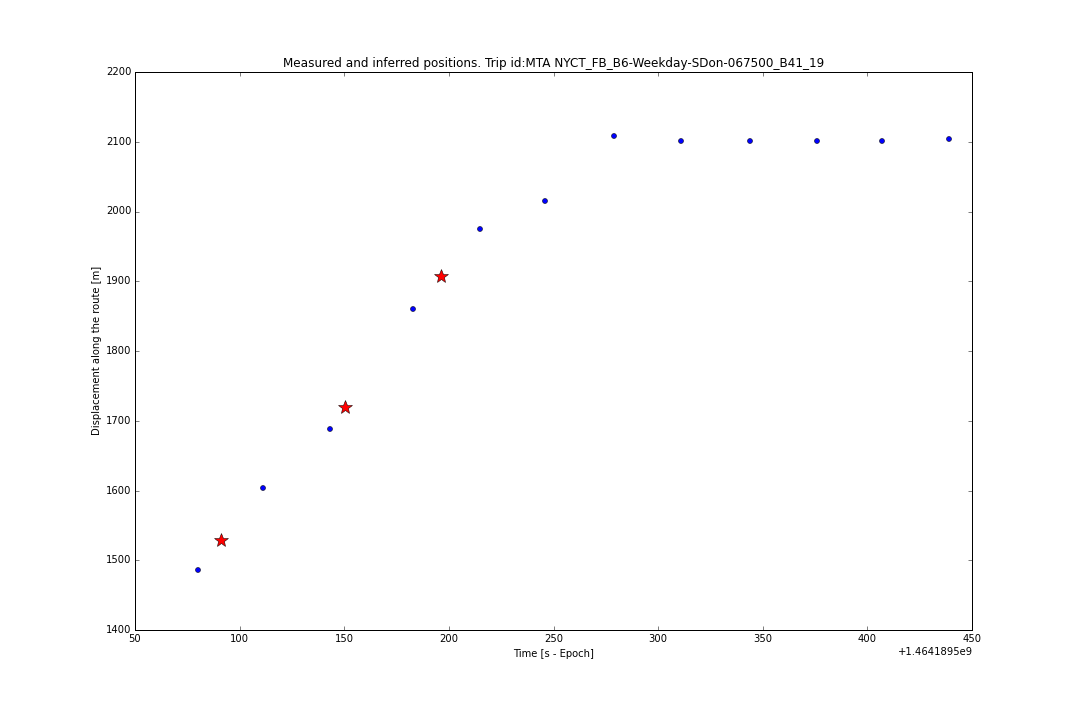
\includegraphics[scale=0.2]{/home/saf537/Documents/CUSP/Capstone/Bus-Capstone/plots/cuteplot}

\subsection{	Statement and Description}
Although demand for public transportation in New York City is growing, bus ridership levels are declining.  Many reasons can explain this, including drops in vehicle speeds and customer perceptions of dependability.  This project focuses on identifying these two factors along the city's MTA operated bus routes with reliability metrics that are relevant to the DOT as the municipal traffic authority.

The DOT keeps records of the MTA vehicle location data through collection via its Bus Time API, but the agency lacks a formal process for compiling and analysing it according to their decision making capabilities (such as those related with road design and traffic management), which substantially differ from the MTA's purposes and reach. Despite the MTA (which is the agency in charge of operations) has internally defined metrics used for scheduling, planning and analysis of the bus service, it pays more attention to the bus level but not to the whole system level, which is more of the interest of the DOT.
 
To help the DOT improve their planning efficiency, this project aims to figure out the dependent variable metrics related to bus performance and reliability, so in a further analysis the agency can analyse the effect of independent variables that affect service quality, such as traffic management and road design. CUSP developed methods for estimating bus travel times and measuring reliability, while performing data quality analysis of the Bus Time data and the MTA schedule data (referred to as \textit{GTFS} in this document for its format, \textit{General Transit Feed Specification}). 

In this project, CUSP collaborated with the DOT to find out what factors are related to bus performance and reliability, by first. Since DOT concerns more about customer satisfaction and is responsible for all the traffic elements in the city, this project will not just limit in bus itself as DOT is able to improve bus performance by controlling other traffic elements, but not only bus operation element. By exploring that, DOT will be able to improve the bus performance and reliability by control certain factors.


\subsection{Goals}

The goals of the project can be summarized as follows:

\begin{enumerate}
\item Perform a thorough data quality assessment on the MTA Bus Time data, 

\item Calculate metrics related to the performance of the buses with respect to their planned schedule.

\item Document the entire process and flexible in the code, so both data quality assessment and reliability measurements are more clearly evaluated by the agency.
\end{enumerate}


The project has been developed following the milestones below:

\begin{itemize}
\item Bibliography review; 
\item Data extraction; 
\item Identification of pitfalls and irregularities in the data generating process;
\item Estimation of the departure and arrival times at bus stops and other locations (in other words, interpolation); 
\item Measurement of bus performance and reliability metrics, with a flexible implementation;
\end{itemize}

\section{Project offerings}

The contributions from our work can be summarized as follows:

\begin{enumerate}
\item The estimation of departure and arrival times based on AVL data for the specific case of Bus Time. 
\item Flexible and potentially novel bus performance metrics for the data set in question.
\item Quality assessment for the Bus Time data.
\item Flexible and reproducible code to allow for further implementations and variations of our analysis.

\end{enumerate}


\section{Approach}

\subsection{Data techniques}

Overall goal of this section: Process can be compared to exchange of daily flat file between MTA and  DOT MTA's Automated Vehicle Location (AVL) data is acquired using a ''get'' request to a web service offered by the MTA to the public.  The web service uses a data standard called Service Interface for Real-Time Information (SIRI).  ''This standard has been adopted by the European standards-setting body CEN, and is not owned by any one vendor, public transportation agency or operator.  It has been implemented in a growing number of different projects by vendors and agencies around Europe. ''

\textbf{[Discuss parameters, API response time, and dependency constant internet connection.  Also discuss accumulated size (each is ~3MB, so an entire year can be >3TB).]}

Per MTA's recommendation, the response data is requested in JSON format (Javascript Object Notation).  JSON offers a flexible structure, for example allowing elements to be stored as hierarchy, or a combination of named and unnamed elements.  JSON does not transform directly to a tabular layout and as a result cannot be imported by typical data analysis tools like Microsoft Access or Excel without first parsing it.
Parsing can be performed using a variety of approaches.  A small program that can be written on almost any personal computer (a macro, or command-line script) may be acceptable for parsing one JSON response, requiring in the order-of-magnitude one second for each JSON.  However this is likely unacceptable for reading and aggregating any meaningful amount of archived JSON response files (entire days, or entire lines over multiple days).  Advanced techniques requiring additional software or hardware, which are explored in this report, can significantly improve processing time by distributing the data across multiple ''workers.''  Regardless of the technique, the extracted data has a straightforward structure, containing text and numerical elements (which can be stored as text), appropriate for storage in a comma-separated values (CSV) file.
A risk that remains to be investigated is incomplete (blank) vehicle data elements.  Faster techniques for parsing of JSON into tabular format require each observation to contain data according to each element extracted.  This results in rectangle-shape data set with no need for validation of each row.

\textbf{]Discuss GTFS. Bus schedules for a given trip include a reference date]}

The SIRI standard calls for date-time representation according to the ISO 8601 standard.  While this can be read directly and used for many typical calculations (for example, elapsed time), it poses a problem when performing any analysis requiring date or time data from the planned schedule for the buses.  Those analysis require both the “true'' date-time element as well as the trip reference date.  Here are two example comparisons of a bus trip's estimated departure from its first stop and the corresponding scheduled departure time. Such a comparison may be used to explain whether bus reliability can be attributed to operational issues such as late departures from the depot.  Note the conversion.

\textbf{(table goes here)}

Note that time zone information is dropped in this conversion.  While this may become problematic if these approaches are applied outside of New York City, the only related risk in this application is to the validity of data from bus trips that occur during Daylight Savings Time shifts.  We elect to deal with those issues tactically rather than add complexity across the entire data set.

\subsection{Measurement techniques}

Two methods are investigated for estimating a vehicle's arrival time at a certain location, such as a bus stop.  Arrival time estimates are the basis for most measurement and identification related to bus reliability, such as vehicle speeds, block times, and headway (which in turn is required for wait assessment).  The first method is use to use a spatial algorithm to identify any datapoints within a certain radius of the location, and make an estimation from within that subset.  Possible calculations on that subset are to take earliest or latest time recorded, the median time recorded, or apply an interpolation to generate a point-estimate at the exact location.  The second method is to apply an interpolation algorithm to all observations from a given vehicle on each trip.  The tradeoff is that this may be more computation than required if not many along the trip are to be estimated.

\textbf{[Processing time - big data techniques required]}


Average vehicle speed is calculated as the difference between estimated arrival times at two points divided by the distance traveled.  A key assumption is that vehicle motion is monotonic (never reversing direction) along any given axis.  Approaches to account for variations in vehicle heading remain to be explored.  The size of the post-processed average speed data set depends on how many point-pairs within each trip are to be calculated.  A dataset reporting the total time (“block time'') and average speed, using only the beginning and end points, would be manageable for most typical desktop application; an entire year would be less than 1GB and could be organized by month, route etc. for easier access.

Calculation of headway also requires estimates of all vehicles' arrival times at a certain location.  Missing estimates (whether due to the data generating process or the estimation algorithm) must be identified, as skipping them may result in an overstatement, based on the time between two or more vehicles' arrivals.  A compiled, processed dataset supporting headway measurement -- that is, containing arrival times of each trip at each stop -- is approximately 2M rows per day of operations.  While the calculations on selected data are simple enough for any typical desktop application, the total size of the database (50-100GB) would require additional hardware and a database management system.

Wait Assessment is a metric used by New York City Transit, defined in the Transit Capacity and Quality of Service Manual as the percentage of actual headways between successive vehicle arrivals that are less than or equal to a given standard.  For example the standard for transit lines operating at XXX scheduled headway is +3 mins during peak hours and +5 mins during off-peak hours.  Peak hours are defined as 6am to 9am and 4pm to 7pm.  Wait Assessment is a simple calculation that can be performed after all headway calculations have been performed for a given location.


Higher-Level Analysis (demonstration of data applied)
Trends along a route - small data (after processing headway data)
Time-period partitions - small data (after processing block time data)
Interruptions - medium data (after processing speed data)
Recurring events - small data (after processing interruptions data)

Big Data Techniques

HDFS
HDFS is a Java-based file system that provides scalable and reliable data storage, and it was designed to span large clusters of commodity servers.
The data must be first uploaded into HDFS to perform big data operations.
Apache Spark 
The total dataset size for one year is over 2 terabytes and stored in nested json format, which is impossible to analyse by any traditional way.
Apache Spark is an open source cluster computing framework that performs parallelized stream computing using multiple CPU cores. Apache Spark is proved to be the fastest open source framework (100 times faster than Hadoop).
Spark SQL
Spark SQL is a Spark module for structured data processing.  Spark SQL relies on Spark Dataframe to operate, while Spark Dataframe is a column structured data collection that can be easily saved to csv for further analysis. 
Spark SQL is efficient and reliable and SQL files are easy to share and cooperate.
Data Schema
The original data is stored in nested json format with lots of redundant information.
The schema function based on Spark Dataframe allows us to understand the data structure in a more distinguishable fashion.


\textbf{(image of the data schema)}

\section{Results and implications for practice}


What is the central message of the project? What do practitioners, city managers, and/or data experts need to know about it?
MTA provides the public API but it is impossible to fully replicate the density of the data they keep internally
Density (time and spatial) may be sufficient for stop and route reliability metrics, but questionable for vehicle speed measurement. (?)
Processing of raw data into useful measurements requires more power than offered by a typical personal computer.
The impact of our results on DOT operations and decision making depends on the to-be-discussed tradeoffs between required accuracy, easy of use, and investment in IT processes. 
Data quality assessment 
Gaps (Time dimension)
Missing observations occur XXXX often
XX% of gaps occur when there is a gap in the API response time, although we cannot rule out an error in the AVL signal
Missing observations ARE/ARE NOT correlated to….
Location (Spatial dimensions)
Coordinates now appear to be projected on to route shape-lines, likely in order to correct for signal noise or simplify distance-along-route calculations
Buses were equipped with Dead Reckoning Units in XXXX, improving location accuracy compared to 2014
Published Bus Stop locations ARE/ARE NOT specific enough to analyze position of stop around intersection/street features
Attributes (line/trip)
Unknown data generating process: Vehicle hardware measures location and time automatically.  The driver inputs, at a minimum, the line and the headsign (destination of the trip).  This process dependency is a potential source of error. It is unknown how additional elements are determined the resulting rate of error.
XX percent of scheduled trips have no reported data in BusTime.  Unknown if that is a technical issue or a ''cancelled trip''
XX percent of trips have BusTime data have no reported data near the beginning or end. Unknown if that is a technical issue or truncated trip.
Potentially running one simple exercise (one line)
Potentially mapping a heatmap of the delay (by one sample metric, does not need to be definitive) by stations/lines
Through the big data technique, we can analyse the whole year data of all the bus lines by using the bus runtime dataset and bus schedule dataset.
Although the dataset given for 2015 is not perfectly collected since missing observations occur quite often, in the large scale, we should be able to predict the delay by using some basic statistical criterias such as standard deviation and mean.
Discussion about the theory
Data Extraction and organization
Our data extraction step picks the useful information from the original json and dumps the redundancies. This step shrinks file size by 30 times and facilitates the future analysis.
Our data organization step turns messy json file into human readable and executable csv that can even been easily analysed through Excel by anyone.

\textbf{(sample table image goes here)}

\textbf{(sample table image goes here)}


[Location estimation methods and their impact on measured reliability]
Compare distributions generated from each method
Compare computation time
Also compare to ground-truth, if available
Recommend, based on the tradeoff (if any)

What are the risks? What are the advantages of the approach?
Risks
Reproducibility - dependence on public API feed
Reproducibility - Framework Dependency such as HDFS and Spark
Big data technique requires HDFS and Spark dependencies. It may take some time and resources to install them
Advantages
Big Data Technique
Open source
HDFS and Spark are both open sourced, which means no extra investment is necessary
Ease to share and reproduce
Since big data is very new technology (Spark is release in few years), we are trying to keep all the data manipulation in simple SQL script. 
DOT can easily change SQL script to fulfill their demand and no extra operation is needed. 
What is required for the approach to be applied in practice/cities today?
Processing of raw data into information (e.g. at stop level) requires big-data techniques for anything beyond small samples (e.g. one day / one line)
Processed data structure is straightforward but still too large for single/dual-core applications.
Data supporting higher-level analysis techniques can be managed with any off-the-shelf database system, including sqLite (open source SQL) or even a series of CSVs
What ethical or privacy considerations are important to the application of the project? 
Implications about causes of variance in bus performance (e.g. infrequent but long dwell time for customer with disability)
Vehicle ID is public and not anonymized. 
While the MTA does not publish archived BusTime data (except for a sample in 2014), we are providing the code for anybody to collect it


\subsection{Conclusions and future work}

\subsubsection{Conclusions}

This project studies the bus performance in New York City and its correlation metrics based on the GPS data offered by MTA. The MTA bus GPS database collects the location of each bus every 30 seconds. After estimating the departure and arrival time for each bus at each stop, we use measurement like headways and wait assessment to figure out the bus performance and reliability. Aimed at helping DOT improve the bus performance efficiently, the metrics focus on not only bus operation element, but also on other traffic aspects. Taking one-year data as our object of study, the data is extremely huge so that big data technology like Spark is widely used in this project. In order to make our work easy to share and reproduce, we choose to use SQL API to manipulate the data, which enable DOT to easily make change by editing the SQL script. 
Conclusion for the model we use. (Introduction, Pros and Cons, Bias)
Model for time estimation
Measurement for bus performance
Method for feature selection
Conclusion for the results we get. (How the result influence the future operation)
Conclusion for the whole analysis process. (Pros and Cons, Bias, Influence)
Pros:
1. Focus on the viewpoint of DOT, the correlation elements we chose not only focus on the bus operation, but also other traffic elements.
2. With such large dataset and big data technique, the result of our analysis is more persuasive compared to traditional sample study.
3. Comparison among models(different models to estimate time as well as to measure performance)
Cons:
1. The choice of elements based on formal studies, the objective of which are not all NYC.
2. Too much assumptions.
3. The departure and arrival time for each bus at each stop comes from indirect approximate methods, it is better for MTA to collect the accurate data to help the model works better.
Influence:
The main goal for us is to figure out the other potential influence factor besides operation to help DOT control and improve bus performance on planning level. Similar methodology and concept could be used in other cities and traffic mode. The big data technology applied in not only traffic analysis but also city wide urban issue offers more reliable result compared with traditional sample studies. 


\subsubsection{Future work}

Feature Selection optimization
Pre study and investigation for NYC
Visualization
Use Javascript to create interactive heat map that predicts the chance of delay of specific bus line or stop
Algorithm optimization
Many analyses right now are not computed using big data technique, which means those analyses are hard to applied in large scale such as one year data. In order to analyse quickly in large scale, we must optimize our algorithms to ensure compatibility with big data techniques such as Spark.
Further Application
Other cities (need to pay attention to data structure, bus GPS data in some cities collect departure and arrival time instead of location)
Other traffic mode (eg. Subway, city bike. Need to pay attention to the different features of each kinds of traffic mode)



\newpage

\section*{References}
\addcontentsline{toc}{section}{References}

Anand, U., 2010. The Elusive Free Radicals, \textit{The Clinical Chemist,} [e-journal] Available at:<\url{http://www.clinchem.org/content/56/10/1649.full.pdf}> [Accessed 2 November 2013]
\newline
\newline

Biology Forums, 2012. \textit{Normal glomerulus. Acute glomerulonephritis.} [online] Available at: <\url{http://biology-forums.com/index.php?action=gallery;sa=view;id=9284}> [Accessed 23 October 2013].
\newline
\newline

Budisavljevic, M., Hodge, L., Barber, K., Fulmer, J., Durazo-Arvizu, R., Self, S., Kuhlmann, M., Raymond, J. and Greene, E., 2003. Oxidative stress in the pathogenesis of experimental mesangial proliferative glomerulonephritis, \textit{American Journal of Physiology - Renal Physiology,} 285(6), pp. 1138-1148.
\newline
\newline

Chien, C., Lee, P., Chen, C., Ma, M., Lai, M. and Hsu, S., 2001. De Novo Demonstration and Co-localization of Free-Radical Production and Apoptosis Formation in Rat Kidney Subjected to Ischemia/Reperfusion, \textit{Journal of the American Society of Nephrology,} 12(5), pp. 973-982.
\newline
\newline

Couser, W., 1993. Pathogenesis of glomerulonephritis, \textit{Kidney International Supplements,} 42, pp. 19-26.
\newline
\newline

De Gasparo, M., 2002. Angiotensin II and nitric oxide interaction, \textit{Heart Failure Reviews,} [e-journal] Available at:<\url{http://www.ncbi.nlm.nih.gov/pubmed/12379820}> [Accessed 26 October 2013]
\newline
\newline

Edinburgh Renal Education Pages, 2012. \textit{Glomerulonephritis} [online] Available at: <\url{http://www.edrep.org/pages/textbook/glomerulonephritis.php}> [Accessed 25 October 2013].
\newline
\newline

Forbes, J., Coughlan, M. and Cooper, M., 2008. Oxidative Stress as a Major Culprit in Kidney Disease in Diabetes, \textit{Diabetes,} 57(6), pp. 1446-1454.
\newline
\newline

Geeky Medics, 2010. \textit{Glomerulonephritis} [online] Available at: <\url{http://geekymedics.com/2010/10/27/glomerulonephritis/}> [Accessed 25 October 2013].
\newline
\newline

Gryglewski, R., Palmer, R., Moncada, S., 1986. Superoxide anion is involved in the break­down of endothelium derived relaxing factor, \textit{Nature,} 320, pp. 454-456.
\newline
\newline

Halliwell, B., 2001. Free Radicals and other reactive species in Disease, \textit{Encyclopedia of Life Sciences,} [e-journal] Available at:<\url{http://web.sls.hw.ac.uk/teaching/level4/bcm1_2/reading/oxidative_stress/files/Oxidative_stress.pdf}> [Accessed 19 October 2013]
\newline
\newline

Huang, H., Patel, P. and Salahudeen, A., 2001. Lazaroid compounds prevent early but not late stages of oxidant-induced cell injury: potential explanation for the lack of efficacy of lazaroids in clinical trials, \textit{Pharmacological Research,} 41(1), pp. 55-61.
\newline
\newline

Klinger, J., Abman, S. and Gladwin, M., 2013. Nitric Oxide Deficiency and Endothelial Dysfunction in Pulmonary Arterial Hypertension, \textit{American Journal of Respiratory and Critical Care Medicine,} 188(6), pp. 639-646.
\newline
\newline

Lindemann, I., Boettcher, J., Oertel, K., Pasternack, R., Heine, A. and Klebe, G. 2012. Inhibitors of Transglutaminase 2: A therapeutic option in celiac disease, \textit{To be Published,} [e-journal + PDB structure] Available at:<\url{http://www.ebi.ac.uk/pdbe-srv/view/entry/3s3s/summary}> [Accessed 24 October 2013]
\newline
\newline

Mayo Clinic, 2011. \textit{Glomerulonephritis} [online] Available at: <\url{http://www.mayoclinic.com/health/glomerulonephritis/DS00503/}> [Accessed 20 October 2013].
\newline
\newline

McCord, J., Roy, R. and Schaffer, S., 1985. Free radicals and myocardial ischemia. The role of xanthine oxidase, \textit{Advances in myocardiology,} [e-journal] Available at:<\url{http://www.ncbi.nlm.nih.gov/pubmed/2982206}> [Accessed 24 October 2013]
\newline
\newline

National Health Service, 2012. \textit{Causes of glomerulonephritis} [online] Available at: <\url{http://www.nhs.uk/Conditions/Glomerulonephritis/Pages/Causes.aspx}> [Accessed 20 October 2013].
\newline
\newline

Niaudet, P., 2013. \textit{Overview of the pathogenesis and causes of glomerulonephritis in children.} [online] Available at: <\url{http://www.uptodate.com/contents/overview-of- \ the-pathogenesis-and-causes-of-glomerulonephritis-in-children}> [Accessed 21 October 2013].
\newline
\newline

Ronco, P., 2013. \textit{Mechanisms of glomerular crescent formation.} [online] Available at: <\url{http://www.uptodate.com/contents/mechanisms-of-glomerular-crescent-formation}> [Accessed 21 October 2013].
\newline
\newline

Rutchik, J., 2013. \textit{Toxic Neuropathy Clinical Presentation.} [online] Available at: <\url{http://emedicine.medscape.com/article/1175276-clinical#a0216}> [Accessed 26 October 2013].
\newline
\newline

R\&D Systems, 2013. \textit{Technical Information. Ischemia/Reperfusion Injury.} [online] Available at: <\url{http://www.rndsystems.com/cb_detail_objectname_SP96_Ischemia.aspx}> [Accessed 28 October 2013].
\newline
\newline

Salahudeen, A., 1999. Free Radicals in Kidney Disease and Transplantation, \textit{Saudi Journal of Kidney Diseases and Transplantation,} 10(2), pp. 137-143.
\newline
\newline

Sarma, A., Mallick, A. and Ghosh, A., 2010. Free Radicals and Their Role in Different Clinical Conditions: An Overview, \textit{International Journal of Pharma Sciences and Research,} 1(3), pp. 182-192.
\newline
\newline

Shah, S., Baliga, R., Rajapurkar, M. and Fonseca, V., 2007. Oxidants in Chronic Kidney Disease, \textit{Journal of the American Society of Nephrology,} 18(1), pp. 16-28.
\newline
\newline

The University of Utah, Unknown. \textit{Glomerulonephritis} [online] Available at: <\url{http://library.med.utah.edu/WebPath/RENAHTML/RENALIDX.html#8}> [Accessed 25 October 2013].
\newline
\newline

Wang, C. and Salahudeen, A., 1994. Cyclosporine nephrotoxicity: attenuation by an antioxidant -inhibitor of lipid peroxidation in-vitro and in-vivo, \textit{Transplantation,} 58, pp. 940-946.
\newline
\newline

Wang, C. and Salahudeen, A., 1995. Lipid peroxidation accompanies cyclosporine nephrotoxicity: effects of vitamin E, \textit{Kidney International,} 47, pp. 927-934.
\newline
\newline

Weiss, S., 1989. Tissue Destruction by Neutrophils, \textit{New England Journal of Medicine,} 320, pp. 365-376.
\newline
\newline


\end{document}

%-------------------------------------------------------------------------------
% SNIPPETS
%-------------------------------------------------------------------------------

%\begin{figure}[!ht]
%	\centering
%	\includegraphics[width=0.8\textwidth]{file_name}
%	\caption{}
%	\centering
%	\label{label:file_name}
%\end{figure}

%\begin{figure}[!ht]
%	\centering
%	\includegraphics[width=0.8\textwidth]{graph}
%	\caption{Blood pressure ranges and associated level of hypertension (American Heart Association, 2013).}
%	\centering
%	\label{label:graph}
%\end{figure}

%\begin{wrapfigure}{r}{0.30\textwidth}
%	\vspace{-40pt}
%	\begin{center}
%		\includegraphics[width=0.29\textwidth]{file_name}
%	\end{center}
%	\vspace{-20pt}
%	\caption{}
%	\label{label:file_name}
%\end{wrapfigure}

%\begin{wrapfigure}{r}{0.45\textwidth}
%	\begin{center}
%		\includegraphics[width=0.29\textwidth]{manometer}
%	\end{center}
%	\caption{Aneroid sphygmomanometer with stethoscope (Medicalexpo, 2012).}
%	\label{label:manometer}
%\end{wrapfigure}

%\begin{table}[!ht]\footnotesize
%	\centering
%	\begin{tabular}{cccccc}
%	\toprule
%	\multicolumn{2}{c} {Pearson's correlation test} & \multicolumn{4}{c} {Independent t-test} \\
%	\midrule	
%	\multicolumn{2}{c} {Gender} & \multicolumn{2}{c} {Activity level} & \multicolumn{2}{c} {Gender} \\
%	\midrule
%	Males & Females & 1st level & 6th level & Males & Females \\
%	\midrule
%	\multicolumn{2}{c} {BMI vs. SP} & \multicolumn{2}{c} {Systolic pressure} & \multicolumn{2}{c} {Systolic Pressure} \\
%	\multicolumn{2}{c} {BMI vs. DP} & \multicolumn{2}{c} {Diastolic pressure} & \multicolumn{2}{c} {Diastolic pressure} \\
%	\multicolumn{2}{c} {BMI vs. MAP} & \multicolumn{2}{c} {MAP} & \multicolumn{2}{c} {MAP} \\
%	\multicolumn{2}{c} {W:H ratio vs. SP} & \multicolumn{2}{c} {BMI} & \multicolumn{2}{c} {BMI} \\
%	\multicolumn{2}{c} {W:H ratio vs. DP} & \multicolumn{2}{c} {W:H ratio} & \multicolumn{2}{c} {W:H ratio} \\
%	\multicolumn{2}{c} {W:H ratio vs. MAP} & \multicolumn{2}{c} {\% Body fat} & \multicolumn{2}{c} {\% Body fat} \\
%	\multicolumn{2}{c} {} & \multicolumn{2}{c} {Height} & \multicolumn{2}{c} {Height} \\
%	\multicolumn{2}{c} {} & \multicolumn{2}{c} {Weight} & \multicolumn{2}{c} {Weight} \\
%	\multicolumn{2}{c} {} & \multicolumn{2}{c} {Heart rate} & \multicolumn{2}{c} {Heart rate} \\
%	\bottomrule
%	\end{tabular}
%	\caption{Parameters that were analysed and related statistical test performed for current study. BMI - body mass index; SP - systolic pressure; DP - diastolic pressure; MAP - mean arterial pressure; W:H ratio - waist to hip ratio.}
%	\label{label:tests}
%\end{table}